This section introduces a system of states, flows between them, and equations
which can be used to describe risk group dynamics
in deterministic compartmental epidemic models.
\par
We denote the size of risk group $i \in [1, \dots, G]$ as $x_i$
and the vector of all $x_i$ as $\bm{x}$.
The total population size is denoted $N = \sum_i {x_i}$,%
\footnote{Here, as in many models, ``total population'' actually refers to
  an age-constrained range.}
and the proportion that each group represents by $\hat{x}_i = x_i / N$.
The rate of population entry overall is denoted $\nu$,
and the rate of exit by $\mu$.
We do not consider disease-attributable death, which may vary by group,
though this should be the subject of future work.
All rates have units \textit{per year}.
The proportion of the entering population who will enter group $i$
is denoted $\hat{e}_i$.
Since the rate of entry $\nu$ is typically expressed as
a proportion of the total size $N$,
we model the theoretical entering population $\bm{e}$ as also having size $N$,
so that $e_i = \hat{e}_i N$.
\par
Turnover transitions can occur between any two groups, in either direction;
therefore we denote the turnover rates as a $G \times G$ matrix $\zeta$,
where $\zeta_{ij}$ corresponds to the transition $x_i \rightarrow x_j$.
An explicit definition is given in Eq.~(\ref{eq:zeta}),
where the diagonal elements are written $*$ since they represent
transitions from a group to itself, which are inconsequential.
\begin{equation}\label{eq:zeta}
\zeta = \left[\begin{array}{cccc}
	         *          & x_1  \rightarrow x_2 & \cdots & x_1 \rightarrow x_G \\[0.5em]
	x_2 \rightarrow x_1 &          *           & \cdots & x_2 \rightarrow x_G \\[0.5em]
	      \vdots        &        \vdots        & \ddots &       \vdots        \\[0.5em]
	x_G \rightarrow x_1 & x_G \rightarrow x_2  & \cdots &          *
\end{array}\right]
\end{equation}
These transition flows and the associated rates
are summarized for $G = 3$ in Figure~\ref{fig:system}.
\begin{figure}
  \centering
  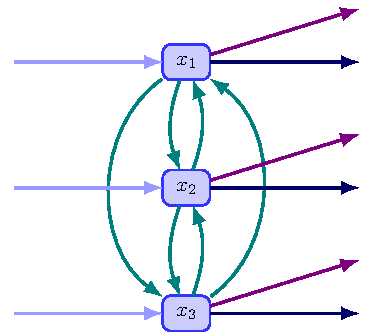
\includegraphics[width=0.4\linewidth]{turnover-system}
  \caption{System of states and flows between them for $G = 3$}
  \label{fig:system}
\end{figure}
% key assumptions
% other stuff?
% ==================================================================================================
\subsection{Parameterization}\label{ss:params}
Next, we explore methods for estimating the values of parameters
in the system described above
($\nu$, $\mu$, $\bm{\hat{x}}$, $\bm{\hat{e}}$, and $\zeta$)
directly from some commonly available sources of data.
% --------------------------------------------------------------------------------------------------
\subsubsection{Total Population Size}\label{sss:params-nu-mu}
The model of total population size over time is defined by
entry and exit rates, $\nu$ and $\mu$, as in:
\begin{subequations}
  \begin{align}
  N(t) &= N_0 {\big(1+\mathcal{G}(t)\big)}^{t} \label{eq:growth-N}\\
  \mathcal{G}(t) &= \nu(t) - \mu(t)              \label{eq:growth-G}
  \end{align}
\end{subequations}
and we note that the average duration of an individual in the model at time $t$
is given by:
\begin{equation} \label{eq:duration-model}
\delta(t) = \mu^{-1}(t)
\end{equation}
Variation in rate of entry across risk groups is captured in $\bm{\hat{e}}$,
and we generally do not stratify rate of exit by activity group
(besides disease-attributable death);
therefore, we can assume that $\nu$ and $\mu$ do not vary across risk groups,
which allows us to derive them with $N(t)$, independent of
the population proportions $\bm{\hat{x}}$, $\bm{\hat{e}}$, and turnover $\zeta$.
\par
The simplest approach assumes a constant population size $N(t) = N_0$,
or a growth rate of zero, yielding $\nu = \mu$.
However, this does not reflect the true positive population growth of most contexts,
and may result in underestimated incidence,
due to the relative reduction in inflow of susceptible individuals.
% verified in code, see:
% https://github.com/c-uhs/turnover/blob/f029bd1/outputs/figs/debug/incidence-nu.gif
\par
Another approach is to fix $\mathcal{G}(t)$ as some constant.
When using this approach, extra care should be taken to ensure
the resulting $N(t)$ matches any available population size estimates to a reasonable degree.
\par
Typically, data will be available for the total size of the population over time $N(t)$,
so the growth rate for each time interval $t_i$
can be derived by rearranging Eq.~(\ref{eq:growth-N}):
\begin{equation}
\mathcal{G}(t_i) = {\left(\frac{N(t_{i+1})}{N(t_{i})}\right)}^{-(t_{i+1}-t_i)} - 1
\end{equation}
All of these approaches help define $\mathcal{G}(t)$, but leave one degree of freedom,
since any choice of $\mu(t)$ can be compensated by $\nu(t)$ to yield the desired $\mathcal{G}(t)$.
However, we can usually leverage the known duration of individuals in the model $\delta(t)$
to choose $\mu(t)$ as in Eq.~(\ref{eq:duration-model}).
This can come from an assumed duration of sexual activity,
or a constant, predefined age range relevant to parameterization.
Then, we can solve for $\nu(t)$ using Eq.~(\ref{eq:growth-G}).
% --------------------------------------------------------------------------------------------------
\subsubsection{Turnover}\label{sss:params-turnover}
% TODO: discuss common approaches - especially turnover is constant, or zero.
% TODO: discuss more the assumptions throughout.
Next, we assume that $\nu(t)$ and $\mu(t)$ are known,
and we focus on resolving $\bm{\hat{e}}(t)$ and $\zeta(t)$.
Similar to above, we will first formulate the problem as a system of equations;
then we will consider which data and assumptions we can leverage to solve the system.
\par
We begin by defining the ``conservation of mass'' equation for a given group $x_i$,
where that the rate of change of the group
is simply the sum of flows in~/~out of the group:
\begin{equation}\label{eq:mass-balance}
\frac{d}{dt}x_i
= \nu \thinspace e_i + \sum_{j}{\zeta_{ji} \thinspace x_j}
- \mu \thinspace x_i - \sum_{j}{\zeta_{ij} \thinspace x_i}
\end{equation}
While Eq.~(\ref{eq:mass-balance}) is written in terms of
absolute population sizes $\bm{x}$ and $\bm{e}$,
it is equivalent to divide through by $N$, yielding a system in terms of
proportions $\bm{\hat{x}}$ and $\bm{\hat{e}}$,
which is often more useful, since $N$ need not be known.
\par
We further assume that the average proportions of each group $\hat{x}_i$ do not change over time.
Therefore, the desired rate of change for risk group $i$
will be equal to the growth of the risk group, $\mathcal{G} x_i$.
Substituting this into Eq.~(\ref{eq:mass-balance}),
and simplifying, we have:
\begin{equation}\label{eq:system}
\nu \thinspace x_i
= \nu \thinspace e_i + \sum_{j}{\zeta_{ji} \thinspace x_j}
- \sum_{j}{\zeta_{ij} \thinspace x_i}
\end{equation}
Now, depending on the number of risk groups, we have
$G$ and $G(G-1)$ unknowns in $\bm{e}$ and $\zeta$, totalling $G^2$ variables to resolve.
We denote these variables as the vector $\bm{\theta} = \left[\bm{e}, \bm{z}\right]$,
where $\bm{z} = \mathrm{vec}_{i \ne j}(\zeta)$;
this allows us to define
a system of linear equations of the form:
\begin{equation}\label{eq:system-matrix}
\bm{b} = A \thinspace \bm{\theta}
\end{equation}
where $A$ is a $G \times G^2 $ matrix
and $\bm{b}$ is a $G$-length vector,
representing the right-hand side and left-hand side of Eq.~(\ref{eq:system}), respectively.
In this form, we can use $A^{-1}\bm{b} = \bm{\theta}$ to solve for $\bm{\theta}$.
\par
Unfortunately, for any $G > 1$, the system is underdetermined by a factor of $G(G-1)$,
meaning there are many combinations of $\bm{e}$ and $\zeta$ which satisfy Eq.~(\ref{eq:system}).
Therefore, we now resume our task of leveraging data and assumptions
to define a unique solution.
\par
Our first tool is another equation.
We note that the duration of time spent in a particular group $\delta_i$
is the inverse of all efferent flow rates:
\begin{equation}\label{eq:duration-group}
\delta_i = {\bigg(\mu + \sum_{j}{\zeta_{ij}}\bigg)}^{-1}
\end{equation}
These durations could be derived from survey data, including for key populations,
or they could be assumed.
Rearranging Eq.~(\ref{eq:duration-group}), we obtain
${\delta_i}^{-1} - \mu = \sum_{j}{\zeta_{ij}}$,
which yields an additional $G$ equations in our linear system -- i.e.\ rows of $A$ and $\bm{b}$.
For $G = 2$, this provides enough constraints to fully determine the system,
as shown in \ref{aa:eqs-turnover} \nameref{aa:eqs-turnover},
but for larger $G$, still more constraints are needed.
\par
The simplest additional constraints can be elements in $\bm{\theta}$ which are directly specified
-- i.e.\ elements of of $\bm{e}$ or $\zeta$.
For example, the proportion of individuals who
move from one risk group to another each year ($\zeta_{ij}$)
may be assumed or derived from data.
Similarly, the distribution of individuals
across risk groups in the entering population $\bm{\hat{e}}$
may be approximated using the proportions among
the lowest age group for which data are available.
In each case, the value specified is appended to $\bm{b}$,
and a row appended to $A$ of the form: $[0,\dots,1,\dots,0]$,
with $1$ in the position of the element in $\bm{\theta}$.
\par
There are, however, two notable caveats to this approach.
First, not all combinations of specified elements will add an equal number of constraints.
Specifying all elements of $\bm{e}$
will only add $G-1$ (not $G$) constraints,
since $\sum \bm{\hat{e}} = 1$, so the final element adds no new information.
Similarly, specifying all elements of $\zeta_{ij}$ for a given $i$
as well as the duration for the group $\delta_i$
will only add $G-1$ (not $G$) constraints,
since Eq.~(\ref{eq:duration-group}) must hold.
%\footnote{Recall that the diagonal elements of $\zeta$ are inconsequential,
%  so only $G-1$ elements of $\zeta_{ij}$ may be specified at all for a given $i$.}
Second, not all combinations of specified values will yield a valid solution,%
\footnote{Even rank-deficient systems be inconsistent.}
and it is unfortunately difficult to anticipate problematic combinations.
\par
Finally, we note that additional constraints may be avoided altogether if we pose the problem
as an optimization problem, namely:
\begin{equation}\label{eq:system-optimize}
\bm{\theta}^{*} = {\arg \min}
\thinspace f(\bm{\theta}),
\quad \textrm{subject to:}
\enspace\bm{b} = A\thinspace\bm{\theta};
\enspace\bm{\theta} \ge 0
\end{equation}
where $f$ is a function such as ${\left|\left| \thinspace\cdot\thinspace \right|\right|}_2$.
However, the choice of $f$ implies a prior on the values of $\bm{\theta}$,
and so introduces bias in the solution.
% ==================================================================================================
\subsection{Previous Approaches}
INP
\begin{floatbox}
  \caption{Common assumptions regarding the dynamics of risk groups}
  \label{box:assumptions}
  \begin{fboxed}
  \begin{enumerate}[leftmargin=1em]
    \item\label{ass:risk-groups}\textbf{Risk Groups:}
    Major demographic groups are stratified by risk of HIV acquisition.
    \begin{enumerate}
      \item\label{ass:risk-groups-no}\textbf{No:} $\G = 1$;
      Major demographic groups are homogeneous in risk of HIV acquisition.
      \item\label{ass:risk-groups-yes}\textbf{Yes:} $\G > 1$;
      Heterogeneity in risk of HIV acquisition within major demographic groups is considered.
    \end{enumerate}
    \item\label{ass:turnover}\textbf{Turnover:}
    Individuals may move between risk groups.
    \begin{enumerate}
      \item\textbf{No:} $\zeta = 0$;
      Individuals do not move between risk groups.
      \item\textbf{Constant:} $\zeta > 0$;
      Individuals move between risk groups at a constant rate.
%      \item\textbf{Dynamic:} $\zeta = f$;
%      Individuals move between risk groups in dynamically.
    \end{enumerate}
    \item\label{ass:pop-growth}\textbf{Population Growth:}
    Increase in the total $\N$ over time.
    \begin{enumerate}
      \item\textbf{No:} $\nu = \mu$;
      Population size $\N$ is constant.
      \item\textbf{Yes:} $\nu > \mu$;
      Population size $\N$ increases, at some constant or data-driven rate.
    \end{enumerate}
  \end{enumerate}
\end{fboxed}

\end{floatbox}

